%
% 2_ggT.tex -- Abschnitt 2 ggT berechnung mit der Tableau Methode
%
% (c) 2020 Prof Dr Andreas Müller, Hochschule Rapperswil
%
% !TEX root = ../../buch.tex
% !TEX encoding = UTF-8
%
\section{Grösster gemeinsamer Teiler (\(\operatorname{ggT}\))
\label{resultante:section:ggT}}
\kopfrechts{Grösster gemeinsamer Teiler (\(\operatorname{ggT}\))}
\subsection*{ggT in der Tableaumethode
\label{resultante:subsection:tableau}}
Für die Berechnung des grössten gemeinsamen Teilers von \(a(X)\) und \(b(X)\) mit \(n = \deg a \geq m = \deg b\) in der Tableaumethode, beginnt mit der Sylvertermatrix \(\operatorname{Syl}(b,a)\).
Das ist die Matrix aus Definition \ref{resultante:definition:Sylvester} in der alle \(m\)-Zeilen des \(a(X)\) Polynoms mit denen des \(b(X)\) Polynoms vertauscht werden.
Auf diese Matrix werden nun \(n-m+1\)-Gauss-Zeilenoperationen angewandt.
Um nun auf die Stufenform der Sylvestermatrix zurück zu kommen, wird auf den Restpolynomen zusätzliche Zeilenoperationen angewant, bis der Rest sich auf jeder Zeile wiederholt.
In den unteren \(m\)-Zeilen ensteht der entsprechende Rest \(r(X)\) der Division von \(a(X)\) und \(b(X)\).
Desweiteren werden die ersten \(n-m+1\) Spalten Nullen enthalten:

\begin{equation*}
    \centering
    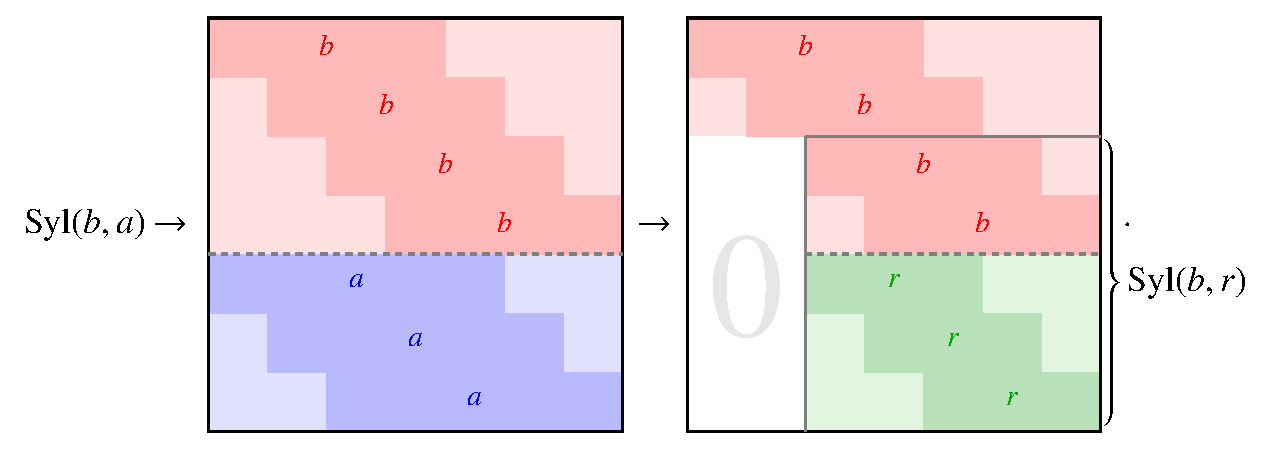
\includegraphics[width=\textwidth]{papers/resultante/pictures/SylvesterTableau.pdf}
    % \caption{britischen Mathematiker James Joseph Sylvester \ref{resultante:jjsylvester}}
    \label{resultante:equation:sylvesterTab}
\end{equation*}

In der rechten unteren Ecke ist nun eine kleinere Sylvestermatrix \(\operatorname{Syl}(b,r)\) entstanden.
Die Polynome in der neuen Sylvestermatrix werden ebenfalls vertauscht und der nächste Rest kann mit derselben Methode berechnent werden.
Das zeigt folgendes Beispiel:

\begin{beispiel}
    Die Vorgehensweise zur ermittlung des grössten gemeinsamen Teilers wird mit Hilfe von \(a(X)=4X^4-7X^3+22X^2-24X+5\) und \(b(X)=8X^3+8X^2-16X\) gezeigt.
    Im ersten Tableau sind die ersten \(4\) Zeilen Kopien von \(b(X)\) und die \(3\) darunter die von \(a(X)\):
    \begin{equation}
        \begin{NiceArray}{*{7}{c}}[cell-space-limits=3pt]
        8 & 8 & -16 & 0 & 0 & 0 & 0 \\
        0 & 8 & 8 & -16 & 0 & 0 & 0 \\
        0 & 0 & 8 & 8 & -16 & 0 & 0 \\
        0 & 0 & 0 & 8 & 8 & -16 & 0 \\
        4 & -7 & 22 & -24 & 5 & 0 & 0 \\
        0 & 4 & -7 & 22 & -24 & 5 & 0 \\
        0 & 0 & 4 & -7 & 22 & -24 & 5 
        \CodeAfter
            \tikz {
                \draw ([xshift=-4pt,yshift=1pt]1-|1) rectangle ([xshift=4pt,yshift=-1pt]8-|8);
                \draw[dashed] ([xshift=-4pt,yshift=1pt]5-|1) -- ([xshift=4pt,yshift=1pt]5-|8);
            }
        \end{NiceArray}
        \,\,\to\,\,
        \begin{NiceArray}{*{7}{c}}[cell-space-limits=3pt]
        1 & 1 & -2 & 0 & 0 & 0 & 0 \\
        0 & 1 & 1 & -2 & 0 & 0 & 0 \\
        0 & 0 & 1 & 1 & -2 & 0 & 0 \\
        0 & 0 & 0 & 1 & 1 & -2 & 0 \\
        0 & 0 & 41 & -46 & 5 & 0 & 0 \\
        0 & 0 & -11 & 30 & -24 & 5 & 0 \\
        0 & 0 & 4 & -7 & 22 & -24 & 5
        \CodeAfter
            \tikz {
                \draw ([xshift=-4pt,yshift=1pt]1-|1) rectangle ([xshift=4pt,yshift=-1pt]8-|8);
                % \draw[dashed] ([xshift=3pt,yshift=1pt]3-|3) -- ([xshift=3pt,yshift=-1pt]8-|3);
                % \draw[dashed] ([xshift=3pt,yshift=1pt]3-|3) -- ([xshift=3pt,yshift=1pt]3-|8);
                \draw[dashed] ([xshift=-4pt,yshift=1pt]5-|1) -- ([xshift=4pt,yshift=1pt]5-|8);
            }
        \end{NiceArray}\,\,\,.
        \label{resultante:equation:step1}
    \end{equation}
    Die Stufenform wird wieder hergestellt indem noch weitere Zeilenoperationen auf den letzten zwei Zeilen angewandt wird:
    \begin{equation}
        \begin{NiceArray}{*{7}{c}}[cell-space-limits=3pt]
        1 & 1 & -2 & 0 & 0 & 0 & 0 \\
        0 & 1 & 1 & -2 & 0 & 0 & 0 \\
        0 & 0 & 1 & 1 & -2 & 0 & 0 \\
        0 & 0 & 0 & 1 & 1 & -2 & 0 \\
        0 & 0 & 41 & -46 & 5 & 0 & 0 \\
        0 & 0 & 0 & 41 & -46 & 5 & 0 \\
        0 & 0 & 0 & 0 & 41 & -46 & 5
        \CodeAfter
            \tikz {
                \draw ([xshift=-4pt,yshift=1pt]1-|1) rectangle ([xshift=4pt,yshift=-1pt]8-|8);
                \draw[dashed] ([xshift=3pt,yshift=1pt]3-|3) -- ([xshift=3pt,yshift=-1pt]8-|3);
                \draw[dashed] ([xshift=3pt,yshift=1pt]3-|3) -- ([xshift=4pt,yshift=1pt]3-|8);
                \draw[dashed] ([xshift=3pt,yshift=1pt]5-|3) -- ([xshift=4pt,yshift=1pt]5-|8);
            }
        \end{NiceArray}\,\,\,.
        \label{resultante:equation:step2}
    \end{equation}
    Im kleineren Tableau unten rechts ist oben das Polynom \(b(X)\) und darunter das Restpolynom \(r(X)=r_1(X)=41X^2-46X+5\).
    Nun werden die beiden Bereiche vertauscht und die gleiche Methode wiederholt:
    \begin{equation}
        \begin{NiceArray}{*{5}{c}}[cell-space-limits=3pt]
        41 & -46 & 5 & 0 & 0 \\
        0 & 41 & -46 & 5 & 0 \\
        0 & 0 & 41 & -46 & 5 \\
        1 & 1 & -2 & 0 & 0 \\
        0 & 1 & 1 & -2 & 0
        \CodeAfter
            \tikz {
                \draw ([xshift=-3pt,yshift=1pt]1-|1) rectangle ([xshift=4pt,yshift=-1pt]6-|6);
                \draw[dashed] ([xshift=-3pt,yshift=1pt]4-|1) -- ([xshift=4pt,yshift=1pt]4-|6);
            }
        \end{NiceArray}
        \,\,\to\,\,
        \begin{NiceArray}{*{5}{c}}[cell-space-limits=3pt]
        1 & -\frac{46}{41} & \frac{5}{41} & 0 & 0 \\
        0 & 1 & -\frac{46}{41} & \frac{5}{41} & 0 \\
        0 & 0 & 1 & -\frac{46}{41} & \frac{5}{41} \\
        0 & 0 & \frac{435}{1681} & -\frac{435}{1681} & 0 \\
        0 & 0 & 0 & \frac{435}{1681} & -\frac{435}{1681}
        \CodeAfter
            \tikz {
                \draw ([xshift=-4pt,yshift=1pt]1-|1) rectangle ([xshift=3pt,yshift=-1pt]6-|6);
                \draw[dashed] ([xshift=1pt]3-|3) -- ([xshift=1pt,yshift=-1pt]6-|3);
                \draw[dashed] ([xshift=1pt]3-|3) -- ([xshift=3pt]3-|6);
                \draw[dashed] ([xshift=1pt]4-|3) -- ([xshift=3pt]4-|6);
            }
        \end{NiceArray}\,\,\,.
        \label{resultante:equation:step3}
    \end{equation}
    Erneut ist der Rest \(r_2(X)=\frac{435}{1681}X-\frac{435}{1681}\) in den unteren Zeilen zu finden.
    Der Subbereich wird erneut vertauscht und der letzte Rest bestimmt:
    \begin{equation}
        \begin{NiceArray}{*{3}{c}}[cell-space-limits=3pt]
        \frac{435}{1681} & -\frac{435}{1681} & 0 \\
        0 & \frac{435}{1681} & -\frac{435}{1681} \\
        1 & -\frac{46}{41} & \frac{5}{41}
        \CodeAfter
            \tikz {
                \draw ([xshift=-3pt,yshift=1pt]1-|1) rectangle ([xshift=3pt,yshift=-1pt]4-|4);
                \draw[dashed] ([xshift=-3pt]3-|1) -- ([xshift=3pt]3-|4);
            }
        \end{NiceArray}
        \,\,\to\,\,
        \begin{NiceArray}{*{3}{c}}[cell-space-limits=3pt]
        1 & -1 & 0 \\
        0 & 1 & -1 \\
        0 & 0 & 0
        \CodeAfter
            \tikz {
                \draw ([xshift=-4pt,yshift=1pt]1-|1) rectangle ([xshift=4pt,yshift=-1pt]4-|4);
                \draw[dashed] ([xshift=2pt,yshift=1pt]3-|3) -- ([xshift=2pt,yshift=-1pt]4-|3);
                \draw[dashed] ([xshift=-4pt,yshift=1pt]3-|1) -- ([xshift=4pt,yshift=1pt]3-|4);
            }
        \end{NiceArray}\,\,\,.
        \label{resultante:equation:step4}
    \end{equation}
    Aus dem Schlusstableau kann der letzte Rest \(r_3(X)=0\) herausgelesen werden.
    In der Zeile darüber ist der normierte grösste gemeinsame Teiler, was dem Rest aus dem vorherigen Schritt entpricht.
    Somit ist \(X-1\) der grösste gemeinsame Teiler von \(a(X)\) und \(b(X)\).
    \label{resultante:beispiel:ggt}
\end{beispiel}

Diese Methode ermöglicht es also, den grössten gemeinsamen Teiler zu bestimmen.
Da sich die Polynome (\(a(X)\) und \(b(X)\) respektive \(b(X)\) und \(r(X)\)) in der Sylvestermatrix jeweils um eine Spalte verschoben wiederholen muss, reicht es aus die erste Zeile auf das Pivot element zu normieren und auf die restlichen Zeilen des Polynoms zu kopieren.
Ausserdem können weitere Zeilenoperationen eingespart werden, indem nur die erste Zeile des Restes berechnet wird und auf den darunter liegenden Zeilen kopiert wird.


\subsection*{Die Determinante der Sylvestermatrix
\label{resultante:subsection:determ}}

Die Vertauschung von Zeilen und die Zeilenoperationen selbst, die zur Berechnung des Restes der Sylvestermatrix nötig sind, ändern die Determinante der Sylvestermatrix nicht.
Lediglich werden \(nm\) Vertauschungen für die Methode benötigt, daher folgt
\begin{equation}
    \det(\operatorname{Syl}(a,b))=(-1)^{nm}\det(\operatorname{Syl}(b,a)).
\end{equation} 
Es kann also höchsten zu einem wechsels des Vorzeichens kommen bei der Determinante.

Der Algorithmus zur Berechnung der Determinante endet sobald der grüne Rest \(=0\) ist oder im braunen Feld (das mit dem \(?\)) eine Zahl steht bleibt.
Ist der Rest \(=0\) ist in der darüber liegenden Zeile der grösste gemeinsame Teiler ein Polynom vom Grad \(\geq1\):
\begin{equation*}
    \centering
    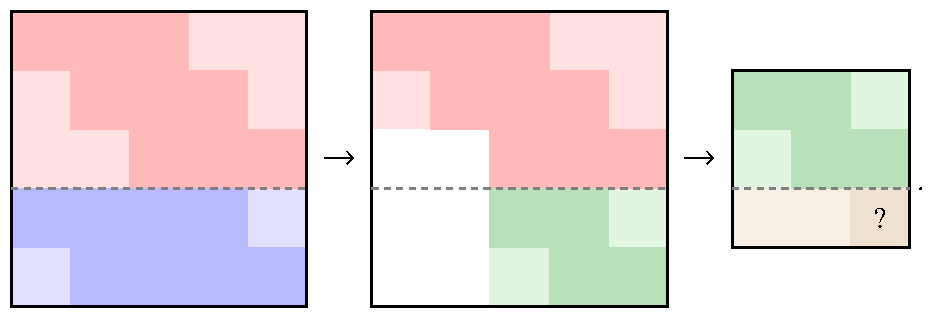
\includegraphics[width=0.8\textwidth]{papers/resultante/pictures/FinalTableau.pdf}
    \label{resultante:equation:finalTab}
\end{equation*}
Falls der letzte Rest im braunen Feld \(\neq0\) übrig bleibt, dann ist der grösste gemeinsame Teiler \(=1\), die beiden Polynome \(a(X)\) und \(b(X)\) sind somit teilerfremd.

Daraus lässt sich ablesen, die Determinante ist genau dann verschieden von Null, wenn die beiden Polynome teilerfremd sind. 
\begin{satz}
    (Resultante und Teiler). Zwei Polynome \(f(X)\) und \(g(X)\) sind genau dann teilerfremd, wenn \(\det(\operatorname{Syl}(f,g))\neq0\) ist.
\end{satz}
\begin{definition}
    (Resultante). Wie bereits in Einleitung (\ref{resultante:equation:definition}) geschrieben. Sind \(f\) und \(g\) Polynome, dann heisst die Determinante der Sylvestermatrix
    \begin{equation*}
        \operatorname{Res}(f,g)=\det(\operatorname{Syl}(f,g))
    \end{equation*}
    die Resultante der Polynome.
    \label{resultante:definition:resultante}
\end{definition}

Folglich ist die Resultante zweier Polynome genau dann gleich Null, wenn sie eine gemeinsame Nullstelle haben.

Das Beispiel \ref{resultante:beispiel:ggt} zeigt, die berechnung der Resultante lässt sich bereits mit Grundlegende Werkzeugen der linearen Algebra umsetzen. 